\documentclass[11pt,a4paper]{article}
% A short version of the paper, written 20 Oct 2026 after the call with Jerome (19 Oct), following his order:
% setting, Markov / not Markov / Markov, BP for the exact score, the grid, three learners, the Laplace chain, the
% Allen-Cahn field. Every number comes from a frozen output; docs/PAPER_CORE_2026-10-20.md gives the source of each,
% and tools/core/audit_paper.py recomputes them.
\usepackage[T1]{fontenc}
\usepackage[utf8]{inputenc}
\usepackage{newtxtext}   % Times text, Computer Modern math: what the ICML class does, and what the figures use
\usepackage{amsmath,amssymb,amsthm}
\usepackage[margin=2.5cm]{geometry}
\usepackage{microtype}
\usepackage{booktabs}
\usepackage{graphicx}
\usepackage[font=small,labelfont=bf]{caption}
\usepackage[round]{natbib}
\usepackage[hidelinks]{hyperref}
\graphicspath{{../figures/}}
\setlength{\parskip}{0.3em}
\renewcommand{\topfraction}{0.9}\renewcommand{\textfraction}{0.07}\renewcommand{\floatpagefraction}{0.8}

\newtheorem{proposition}{Proposition}
\newcommand{\E}{\mathbb{E}}
\newcommand{\N}{\mathcal{N}}
\newcommand{\va}{\mathbf{a}}
\newcommand{\vx}{\mathbf{x}}
\newcommand{\vz}{\mathbf{z}}

\title{Exact diffusion scores for Markov data\\ with belief propagation}
\author{Giovanni Mantovani \and J\'er\^ome Garnier-Brun \and Marc M\'ezard}
% author list and order to be confirmed
\date{Draft, 20 October 2026}

\begin{document}
\maketitle

\begin{abstract}
A diffusion model learns the score of noisy data. To understand what a network learns, one needs the exact score, which is
rarely available. We study data generated by a stationary first-order Markov chain. Gaussian noise destroys the Markov
property of the data at intermediate noise levels, but the posterior of the clean chain given the noisy one is still a chain.
Belief propagation on this chain therefore gives the exact score for any transition kernel, also when no closed form exists,
and we compute it on a grid. When the kernel is unknown, we learn it from noisy sequences alone by expectation--maximisation,
with belief propagation as the E-step. On a linear chain with Laplace noise, this estimator trained on 32 sequences is more
accurate than a convolutional network trained by denoising score matching on 2048. On snapshots of the stochastic
Allen--Cahn equation, a kernel with five parameters reaches 3 to 17\% of the error of the best linear denoiser, and its
parameters give back the temperature and the double-well potential of the model.
\end{abstract}

%=====================================================================================================================
\section{Introduction}

Diffusion models generate data by reversing a noising process, and the only object they learn is the score, the gradient of
the log-density of the noisy data at each noise level \citep{sohl2015deep,ho2020denoising,song2021scorebased}. A trained
network does not reproduce its training set: it generalises \citep{kadkhodaie2024generalization}. To understand what it
learns, it helps to know the exact score of the data distribution. The exact score explains the dynamical regimes of the
backward process \citep{biroli2024dynamical} and when a model memorises \citep{bonnaire2025memorize}. These results use
simple data models, each chosen to isolate one feature of real data: Gaussian mixtures for multimodality, trees for
hierarchy \citep{sclocchi2025phase,garnierbrun2024transformers}.

Here the feature is order and locality. We take data generated by a stationary first-order Markov chain, a sequence in which
each value depends only on the previous one. We ask what can be done with the exact score when the data are Markov. Three
observations organise the paper, and Figure~\ref{fig:summary} shows one panel for each.

First, the noise breaks the Markov property. For a Gaussian chain the precision matrix of the noisy data is tridiagonal
without noise, dense at intermediate noise, and close to diagonal at large noise (panel a). Second, the posterior of the
clean chain given the noisy one is still a chain, so belief propagation (BP) computes the exact score. With the kernel learned
from noisy data by expectation--maximisation (EM), this estimator needs far fewer samples than a network (panel b). Third, the
method works on data from a physical model, snapshots of the stochastic Allen--Cahn equation, where the kernel has no closed
form and five parameters suffice (panel c).

\begin{figure}[t]
\centering
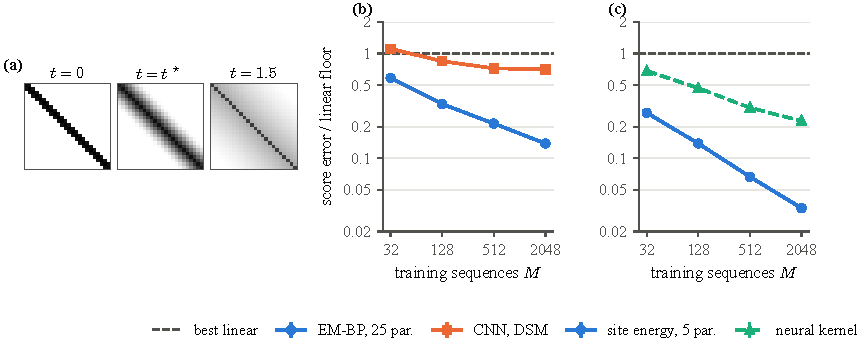
\includegraphics[width=\textwidth]{fig1-summary.pdf}
\caption{(a) Absolute values of the precision matrix $Q_t$ of a noisy Gaussian chain ($\rho=0.85$, $L=24$, one logarithmic grey
scale for the three panels) at $t=0$, at $t^\star=0.075$ where the entries beyond the first off-diagonal are largest, and at
$t=1.5$, where the off-diagonal entries are below $4\%$ of the diagonal. (b) Laplace
chain: score error of EM--BP and of a convolutional network trained by denoising score matching, divided by the error of the
best linear denoiser, against the number $M$ of training sequences. (c) The same for snapshots of the stochastic Allen--Cahn
equation, with a five-parameter kernel and with a neural kernel inside BP. Mean over seeds, bars one standard error.}
\label{fig:summary}
\end{figure}

Our contributions are the following.
\begin{itemize}
\item For any first-order chain observed through Gaussian noise, the exact score at every noise level is given by BP on a
grid, with an error that we measure and that is at round-off for smooth kernels (Section~\ref{sec:bp}).
\item The kernel can be learned from noisy sequences alone by EM through BP. With the right family of kernels this estimator
beats a network trained on $64$ times more sequences (Section~\ref{sec:laplace}).
\item On the Allen--Cahn field the learned kernel is a physical model: its temperature and potential can be read off it, and
two identities give the temperature also from a neural kernel (Section~\ref{sec:field}).
\end{itemize}

%=====================================================================================================================
\section{Noise breaks the Markov property}
\label{sec:setting}

The clean data are sequences $\va=(a_1,\dots,a_L)$ from a stationary chain,
\[
p(\va)=\pi(a_1)\prod_{i=1}^{L-1}K(a_{i+1}\mid a_i),
\]
with transition kernel $K$ and stationary law $\pi$, standardised to unit variance. The noising process is the
Ornstein--Uhlenbeck process, so at time $t$
\[
\vx=\alpha_t\va+\sqrt{\Delta_t}\,\vz,\qquad \alpha_t=e^{-t},\quad \Delta_t=1-e^{-2t},\quad \vz\sim\N(0,I).
\]
The score $S_t(\vx)=\nabla_\vx\log p_t(\vx)$ is all a diffusion model needs, and by Tweedie's formula
\citep{robbins1956empirical,efron2011tweedie} it is a function of the posterior mean,
\begin{equation}
S_t(\vx)=-\frac{\vx-\alpha_t\,\E[\va\mid\vx]}{\Delta_t}.
\label{eq:tweedie}
\end{equation}

The simplest chain is Gaussian, $a_{i+1}=\rho a_i+\sqrt{1-\rho^2}\,\varepsilon_i$ with $\varepsilon_i\sim\N(0,1)$. Its
covariance is $\Sigma_0=(\rho^{|i-j|})_{ij}$ and its precision $Q_0=\Sigma_0^{-1}$ is tridiagonal: this is the Markov
property written in algebra. The noisy data are Gaussian with covariance $\Sigma_t=\alpha_t^2\Sigma_0+\Delta_tI$ and their
score is linear, $S_t(\vx)=-Q_t\vx$ with $Q_t=\Sigma_t^{-1}$. At $t=0$, $Q_t$ is tridiagonal; as $t\to\infty$ it tends to the
identity; in between it is dense (Figure~\ref{fig:summary}a). The noisy sequence is no longer a Markov chain, and the score at
one site depends on the whole sequence. For a Gaussian chain this costs nothing, since the score is a matrix product. For any
other chain the score is nonlinear and has no closed form. The next section shows how to compute it.

%=====================================================================================================================
\section{The exact score by belief propagation}
\label{sec:bp}

Given $\vx$, the posterior of the clean sequence is
\[
p(\va\mid\vx)\;\propto\;\pi(a_1)\prod_{i=1}^{L-1}K(a_{i+1}\mid a_i)\prod_{i=1}^{L}\ell_i(a_i),\qquad
\ell_i(a)=\N(x_i;\alpha_t a,\Delta_t).
\]
The noise acts on each site separately, so the posterior is again a chain. Its factor graph is a tree, and on a tree belief
propagation, the sum--product algorithm \citep{pearl1988probabilistic,kschischang2001factor,mezard2009information}, is
exact. It sends one message forward and one backward along the chain,
\begin{align*}
m^{\rightarrow}_{1}(a)&=\pi(a), & m^{\rightarrow}_{i+1}(a)&=\int K(a\mid b)\,\ell_i(b)\,m^{\rightarrow}_{i}(b)\,db,\\
m^{\leftarrow}_{L}(a)&=1, & m^{\leftarrow}_{i-1}(b)&=\int K(a\mid b)\,\ell_i(a)\,m^{\leftarrow}_{i}(a)\,da,
\end{align*}
and the marginal of site $i$ is $p(a_i\mid\vx)\propto m^{\rightarrow}_i(a_i)\,\ell_i(a_i)\,m^{\leftarrow}_i(a_i)$. Its mean,
put into \eqref{eq:tweedie}, gives the exact score at every site. The only input is the kernel $K$; no closed form of the score
is needed. This is the same forward--backward recursion as for hidden Markov models \citep{rabiner1989tutorial}, here with a
continuous hidden state.

\textbf{The grid.} Each message is a function on $\mathbb R$. We represent it by its values on $N_g$ equally spaced points
of $[-A,A]$ and replace the integrals by the trapezoid rule, so that one update is a matrix--vector product with the matrix
$K(u_j\mid u_k)$. A sequence costs $O(LN_g^2)$ operations. We use $N_g=401$ and $A=8$ (in units of the standard deviation)
throughout, and we measure the error this causes. On a Gaussian chain the grid score matches the closed form to $2\times10^{-13}$
from $81$ points on; on the Allen--Cahn chain of Section~\ref{sec:field} it matches a $1601$-point reference to
$2\times10^{-11}$ at $101$ points (Appendix~\ref{app:grid}). On kernels with a kink, such as the Laplace noise of
Section~\ref{sec:laplace}, the error decreases more slowly, as a power of $N_g$; it is $9\times10^{-6}$ at $401$ points, well
below every learning error we report.

\textbf{Why not Gaussian messages.} A natural alternative to the grid is to keep each message Gaussian, as approximate message
passing does in dense models \citep{thouless1977solution,donoho2009message}. On a chain this gives nothing beyond a linear
estimator.

\begin{proposition}
Let the kernel be linear and Gaussian, $K(a'\mid a)=\N(a';\rho a,q)$, and $\pi$ Gaussian. Then every BP message is
Gaussian, its variance does not depend on $\vx$ and its mean is linear in $\vx$. Hence $\E[\va\mid\vx]=H_t\vx$ for a fixed
matrix $H_t$, and the score is linear.
\end{proposition}

\begin{proof}
If $m^{\rightarrow}_i=\N(\mu_i,v_i)$, one forward step gives $m^{\rightarrow}_{i+1}=\N(\mu_{i+1},v_{i+1})$ with
\[
v_{i+1}=\rho^2\big(v_i^{-1}+\alpha_t^2/\Delta_t\big)^{-1}+q,\qquad
\mu_{i+1}=\rho\,\big(v_i^{-1}+\alpha_t^2/\Delta_t\big)^{-1}\big(\mu_i/v_i+\alpha_t x_i/\Delta_t\big).
\]
The variances never involve $\vx$, and the means are linear in $\vx$ by induction. The backward messages are the same, and a
marginal is the product of three Gaussians.
\end{proof}

Replacing a non-Gaussian chain by Gaussian messages therefore gives a linear estimator, and no linear estimator beats the
linear minimum mean-square-error (LMMSE) one, $\E^{\rm lin}[\va\mid\vx]=\alpha_t\Sigma_0\Sigma_t^{-1}\vx$, whose score is
$-\Sigma_t^{-1}\vx$, the score of the Gaussian with the same covariance as the data. We call its error the \emph{linear floor}
and report every error relative to it. A ratio below one means that the estimator uses structure that no linear denoiser can
use.

%=====================================================================================================================
\section{Learning the kernel through the noise}
\label{sec:learning}

In practice $K$ is unknown, and we have noisy sequences only. Each of the $M$ training sequences is observed once, at one of
twelve noise levels $t\in[0.05,3]$ (log-spaced), the sequences being split evenly between the levels. We fit a parametric
kernel $K_\theta$ by maximising the likelihood of the noisy data, which BP computes as a by-product. The EM algorithm
\citep{dempster1977maximum} does this with BP as the E-step. From the current $\theta$, BP gives the posterior of every pair
$(a_i,a_{i+1})$; summed over sites and sequences, these give the expected pair counts $\Xi(a,a')$ on the grid. The M-step
maximises $\sum_{a,a'}\Xi(a,a')\log K_\theta(a'\mid a)$. The gradient of the noisy-data log-likelihood is the posterior
average of $\nabla_\theta\log K_\theta$ (Fisher's identity), so the procedure is maximum likelihood without ever seeing a
clean sequence. The learned kernel is then used in BP and \eqref{eq:tweedie} to give the score.

We compare three estimators, each knowing less about the data than the previous one.
\begin{enumerate}
\item \textbf{EM--BP with a kernel family of the right shape.} For the linear chain of Section~\ref{sec:laplace},
$K_\theta(a'\mid a)=\sum_{c=1}^{8}w_c\,\N(a'-\rho a;\mu_c,s_c^2)$, a linear drift with a mixture of eight Gaussians as noise
(25 parameters). For the Allen--Cahn field, the five-parameter kernel of Section~\ref{sec:field}.
\item \textbf{EM--BP with a neural kernel.} A mixture density network \citep{bishop1994mixture},
\[
K_\theta(a'\mid a)=\sum_{c=1}^{4}w_c(a)\,\N\big(a';\mu_c(a),s_c(a)^2\big),
\]
whose weights, means and variances are outputs of a small network (two hidden layers of 32 units, 1{,}516 parameters). It
assumes only that the data are Markov.
\item \textbf{A score network.} A convolutional network trained by denoising score matching
\citep{vincent2011connection,ho2020denoising}: at every step a clean training sequence, a noise level and the noise are drawn
afresh. It assumes nothing about the data except locality, and it sees the clean sequences, which EM--BP never does.
\end{enumerate}
Each estimator stops at the checkpoint with the lowest score error on a validation set. The error of an estimator is the
relative score error
$R=\big(\sum\|\hat S_t(\vx)-S_t(\vx)\|^2/\sum\|S_t(\vx)\|^2\big)^{1/2}$, summed over 2048 test sequences and the twelve levels,
with the reference $S_t$ from BP with the true kernel. Details are in Appendix~\ref{app:protocol}.

%=====================================================================================================================
\section{The Laplace chain}
\label{sec:laplace}

We take $a_{i+1}=\rho a_i+\varepsilon_i$ with Laplace noise $\varepsilon_i$ of variance $1-\rho^2$, $\rho=0.85$ and $L=32$.
The chain is Markov and close to the Gaussian one, but its score is nonlinear and has no closed form. The linear floor is
$R=0.167$. Figure~\ref{fig:laplace}a shows the three estimators against the number of training sequences, over 16 seeds.

\begin{figure}[t]
\centering
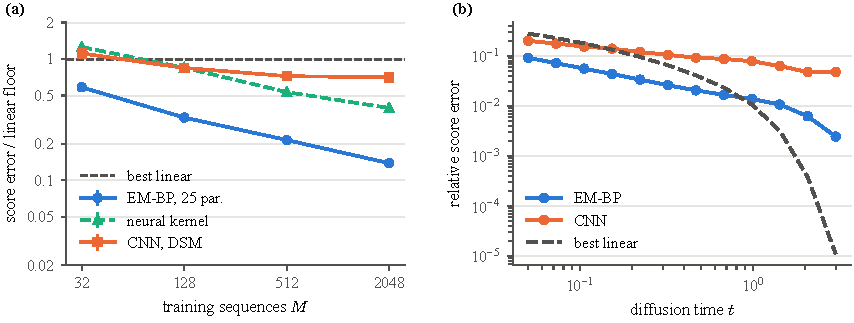
\includegraphics[width=\textwidth]{fig3-laplace.pdf}
\caption{Laplace chain ($\rho=0.85$, $L=32$). (a) Score error divided by the linear floor against the number of training
sequences, for EM--BP with the 25-parameter kernel, EM--BP with a neural kernel, and a convolutional network trained by
denoising score matching. (b) Score error per noise level at $M=128$.}
\label{fig:laplace}
\end{figure}

EM--BP is below the floor already at $M=32$ (ratio $0.59$) and reaches $0.14$ at $M=2048$. The network is above the floor at
$M=32$ ($1.11$) and levels off near $0.71$. With $32$ sequences EM--BP is more accurate than the network with $2048$. The
convolutional network is not the strongest architecture on this task: among six that we tried, the best reaches $R=0.060$ at
$M=2048$, still above EM--BP at $M=128$ ($R=0.055$). The neural kernel lies between the two at large $M$ ($0.39$ at $2048$)
but is above the floor at $M=32$: a free conditional density needs data that a parsimonious family does not.

Panel b separates the noise levels. EM--BP is more accurate than the network at every level. The linear floor is better than
the network above $t\approx0.15$ and better than EM--BP above $t\approx1$; there the noisy data are nearly Gaussian, the true
score is nearly linear, and the small error of a learned kernel is what remains.

%=====================================================================================================================
\section{The stochastic Allen--Cahn field}
\label{sec:field}

\textbf{The model.} The stochastic Allen--Cahn equation \citep{allen1979microscopic},
$\partial_\tau\phi=\partial_x^2\phi-V'(\phi)+\sqrt{2\Theta}\,\eta(x,\tau)$ with $V(\phi)=(\phi^2-1)^2/4$ and space--time white
noise $\eta$, has the stationary law $\propto e^{-H[\phi]/\Theta}$ with $H[\phi]=\int[\tfrac12(\partial_x\phi)^2+V(\phi)]\,dx$. On a
lattice of spacing $h$ the energy is $\sum_i[(\phi_{i+1}-\phi_i)^2/2h+hV(\phi_i)]$, a sum of nearest-neighbour terms, so a
spatial snapshot is exactly a first-order Markov chain in the site index. Its kernel comes from the transfer operator
\[
T(\phi,\phi')=\exp\Big(-\frac{h}{2\Theta}\big[V(\phi)+V(\phi')\big]-\frac{(\phi'-\phi)^2}{2\Theta h}\Big),\qquad
K(\phi'\mid\phi)=\frac{T(\phi,\phi')\,\psi_0(\phi')}{\lambda_0\,\psi_0(\phi)},
\]
with $\lambda_0$ the largest eigenvalue of $T$ and $\psi_0$ its eigenfunction \citep{scalapino1972statistical}. The chain is
reversible, the stationary law is $\psi_0^2$, the partition function of $L$ sites satisfies $\log Z_L=L\log\lambda_0+O(1)$, and the
correlation length is
$\xi=1/\log(\lambda_0/\lambda_1)$ sites. For a quadratic $V$ these quantities have a closed form; for the double well they do
not, since the continuum limit is the Schr\"odinger problem of a quartic double well
\citep{krumhansl1975dynamics,khare1997exact}. We compute them by a dense eigensolve, which converges to $10^{-13}$ and reproduces
the Gaussian closed form to $2\times10^{-14}$ (Appendix~\ref{app:logz}). Cold fields are made of domains near $\phi=\pm1$
separated by kinks.

We use six cells: $\Theta\in\{0.3,0.5,1,2\}$ with $h$ chosen so that $\xi\approx6$ sites ($L=32$), and $h\in\{1,\tfrac12,\tfrac14\}$
at $\Theta=0.3$ with the physical length fixed ($L=32,64,128$).

\textbf{A five-parameter kernel.} The lattice energy is a quadratic bond plus a quartic site term, so the pair energy
\[
W_\theta(a,a')=\frac{(a'-a)^2}{2\gamma}+f(a)+f(a'),\qquad f(a)=\sum_{m=1}^{4}c_m a^m,
\]
with five parameters $(\gamma,c_1,\dots,c_4)$, contains the true model exactly ($a=\phi/s$ is the standardised field). Its kernel
is obtained from $e^{-W_\theta}$ as above, by one eigensolve on the grid. We call it the \emph{site-energy kernel}. The mixture
kernel of Section~\ref{sec:laplace} is misspecified here: its drift is linear, and a linear drift cannot hold a domain.

\textbf{Results.} Table~\ref{tab:field} and Figure~\ref{fig:summary}c give the errors. At $M=2048$ the site-energy kernel is at
$3$ to $17\%$ of the linear floor on every cell, the neural kernel at $23$ to $84\%$, and the mixture kernel at the floor
($1.00$ to $1.02$). With $M=32$ sequences the site-energy kernel is already at $24$ to $28\%$ of the floor on the three cells at
$\Theta=0.3$; on the two hottest cells, where the field is closer to Gaussian, it needs $M=128$ to go below the floor.

\begin{table}[h]
\centering\small
\caption{Score error divided by the linear floor on the six field cells; mean over 16 seeds for the kernels and 8 for the network. Site: the five-parameter site-energy kernel; neural: the neural kernel inside BP; CNN: the network trained by denoising score matching.}
\label{tab:field}
\begin{tabular}{lcccccc}
\toprule
 & \multicolumn{3}{c}{$M=32$} & \multicolumn{3}{c}{$M=2048$} \\
\cmidrule(lr){2-4}\cmidrule(lr){5-7}
cell & site & neural & CNN & site & neural & CNN \\
\midrule
$\Theta=0.3$, $h=1$ & 0.27 & 0.68 & 0.53 & 0.03 & 0.23 & 0.39 \\
$\Theta=0.3$, $h=\tfrac12$ & 0.28 & 0.73 & 0.74 & 0.04 & 0.31 & 0.57 \\
$\Theta=0.3$, $h=\tfrac14$ & 0.24 & 0.97 & 1.08 & 0.03 & 0.42 & 0.79 \\
$\Theta=0.5$ & 0.66 & 1.30 & 1.35 & 0.07 & 0.42 & 0.84 \\
$\Theta=1$ & 1.37 & 2.85 & 2.61 & 0.14 & 0.74 & 1.72 \\
$\Theta=2$ & 1.43 & 3.83 & 3.68 & 0.17 & 0.84 & 2.44 \\
\bottomrule
\end{tabular}
\end{table}


\textbf{Reading the physics off a kernel.} Every kernel built from a pair energy of the form $W$ above, whatever the site term
$f$, satisfies two identities:
\[
\frac{\partial^2\log K(a'\mid a)}{\partial a\,\partial a'}=\frac{1}{\gamma},\qquad\qquad f(a)=-\tfrac12\log K(a\mid a)+\text{const}.
\]
The first holds because $\log K$ is the bond plus a function of $a$ plus a function of $a'$; the second because the bond
vanishes on the diagonal. With $\gamma=\Theta h/s^2$ they give the temperature $\hat\Theta=\hat\gamma s^2/h$ and the potential
$\hat V(\phi)=(2\hat\Theta/h)\hat f(\phi/s)$. For the site-energy kernel this is its own parametrisation: at $M=2048$ on the base
cell ($\Theta=0.3$, $h=1$) the median $\hat\Theta/\Theta$ over seeds is $1.000$ and the barrier is $0.248$ (true value $0.25$).

The identities use no parameter of the kernel, so they apply to the neural kernel too, where the mixed derivative is no
longer constant and we average it under the kernel's stationary pair law. The temperature comes back within $10\%$ on all six
cells at $M=2048$ ($\hat\Theta/\Theta$ from $0.91$ to $1.00$). The potential comes back on the base cell (barrier $0.20$;
Figure~\ref{fig:readings}a) but not on fine or hot lattices, where the factor $2\Theta/h$, up to $27$, multiplies the error of
the kernel's diagonal. A network that knows only that the data are Markov thus recovers part of the physics.

\begin{figure}[t]
\centering
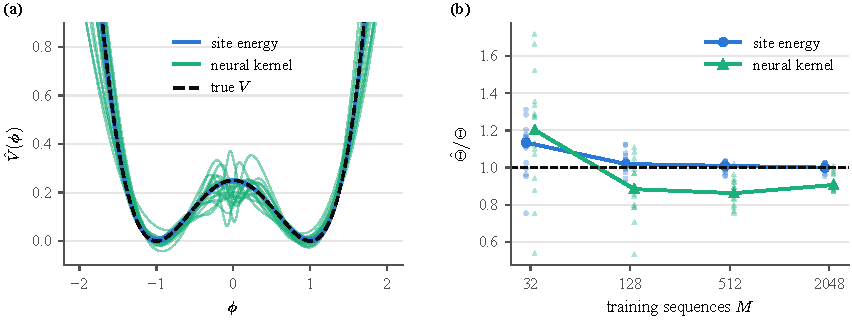
\includegraphics[width=\textwidth]{fig4-field-readings.pdf}
\caption{The physics read off kernels learned from noisy data, base cell. (a) The potential from the diagonal of the kernel,
one curve per seed (16), $M=2048$, for the site-energy kernel and the neural kernel; dashed, the true double well. (b) The
temperature from the mixed derivative of $\log K$; points are seeds, lines join the medians.}
\label{fig:readings}
\end{figure}

%=====================================================================================================================
\section{Discussion}
\label{sec:discussion}

When data are Markov, the exact score is within reach even though the noisy data are not Markov: BP on the posterior chain
computes it for any kernel, and EM through BP learns the kernel from noisy data alone. The advantage over a network is data
efficiency. A kernel with five or 25 parameters cannot memorise even one training sequence of 32 values, and it reaches errors
that a network does not reach with $64$ times more data. On the Allen--Cahn field the learned parameters are the temperature
and the potential of the model.

The method has limits. The data are one-dimensional sequences with first-order dependence. The kernel family is a modelling
choice: the mixture kernel that works on the linear chain fails on the Allen--Cahn field. The neural kernel removes this
choice at the price of more data. The grid costs $N_g^2$ per site, and a very irregular kernel would need more points.
Checkpoints were selected with the exact score on a validation set; with the held-out likelihood instead, which needs no exact
score, the site-energy kernel is at 4 to 23\% of the floor instead of 3 to 17\%.

Two directions follow. One is model inference: from a few noisy time series of interacting units, a Markov kernel with few
parameters can be learned and read. The other is to ask whether networks trained on Markov data learn to implement BP, as they
do on trees \citep{garnierbrun2024transformers,mei2024unets}.

\bibliographystyle{plainnat}
\bibliography{refs}

%=====================================================================================================================
\appendix
\section{Accuracy of the grid}
\label{app:grid}

\begin{figure}[h]
\centering
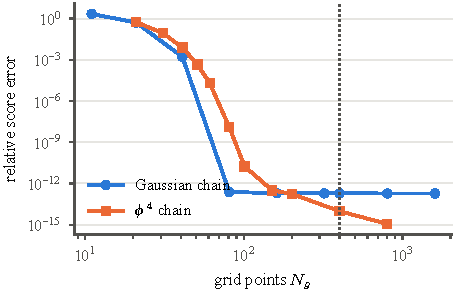
\includegraphics[width=0.55\textwidth]{fig2-grid.pdf}
\caption{Relative score error of grid BP against the number of grid points, on $[-8,8]$: the Gaussian chain ($\rho=0.85$)
against its closed-form score, and the Allen--Cahn base cell against a $1601$-point reference; maximum over noise levels.
Dotted: $N_g=401$.}
\label{fig:grid}
\end{figure}

For smooth kernels the error falls faster than any power of $N_g$ and reaches round-off by $81$ points (Gaussian) and $151$
points (Allen--Cahn). For the Laplace chain, whose kernel has a kink, the error against a $3201$-point reference on a wider
domain is $4\times10^{-5}$ at $201$ points and $9\times10^{-6}$ at $401$.

\section{\texorpdfstring{$\log Z$}{log Z} and the correlation length}
\label{app:logz}

For a chain of $L$ sites, $\log Z_L=L\log\lambda_0+O(1)$. Table~\ref{tab:logz} gives $\log\lambda_0$ and $\xi$ at $h=1$. They change
by less than $2\times10^{-13}$ from $2401$ to $4801$ quadrature points on $[-12,12]$; with $V$ replaced by a quadratic potential the
same solver matches the closed form $\lambda_0=\sqrt{2\pi/(a+c)}$, $a=hk/2\Theta+1/\Theta h$, $c=\sqrt{a^2-(\Theta h)^{-2}}$, to
$2\times10^{-14}$. As $\Theta$ falls, $\log\lambda_0$ approaches the value for a single harmonic well and on fine lattices
$\xi$ grows like $e^{E/\Theta}$ with a fitted $E=0.99$, close to the energy of one kink in the continuum, $2\sqrt2/3\approx0.94$.

\begin{table}[h]
\centering\small
\caption{Free energy per site and correlation length of the lattice field, $h=1$.}
\label{tab:logz}
\begin{tabular}{lccccccc}
\toprule
$\Theta$ & 0.2 & 0.3 & 0.5 & 0.7 & 1 & 1.5 & 2 \\
\midrule
$\log\lambda_0$ & $-0.467$ & $-0.186$ & 0.161 & 0.362 & 0.550 & 0.737 & 0.857 \\
$\xi$ (sites) & 19.47 & 6.08 & 2.75 & 1.98 & 1.53 & 1.21 & 1.06 \\
\bottomrule
\end{tabular}
\end{table}


\section{Protocol}
\label{app:protocol}

\textbf{Data.} For each seed: $M$ training sequences, 1024 validation and 2048 test sequences, each test sequence noised at all
twelve levels. Laplace chain: 16 seeds. Allen--Cahn field: 16 seeds for the kernels, 8 for the network.

\textbf{EM--BP.} Up to 1200 EM iterations, checkpoints along the way, the one with the lowest validation error kept. The
mixture kernel starts from $\rho=0.3$; the neural kernel's M-step is one Adam step with backtracking on the M-step objective, so each EM iteration still increases
the likelihood; the site-energy
kernel's M-step is a quasi-Newton step with the gradient of the eigensolve from first-order perturbation theory.

\textbf{Network.} One convolution of width $2r+1$ with 64 channels, a sinusoidal embedding of $t$ added to it, then two
pointwise layers with $\tanh$, predicting the noise $\vz$ at every site. Radius $r=4$ on the Laplace chain (5{,}505 parameters). On the field $r=2,4,8$ at $h=1,\tfrac12,\tfrac14$ (the same physical
reach) and $r=4$ on the three hotter cells (128 channels at $\Theta=0.5$), chosen on two development seeds. Adam with learning
rate $10^{-3}$, batch 64, gradient clipping at 1; 32{,}000 steps on the Laplace chain and 64{,}000 on the field, checkpoints at
powers of two from 500 steps.

\section{Speciation, site by site}
\label{app:speciation}

As $t$ decreases during generation, the posterior of a cold field commits each site to one well. We followed exact
Ornstein--Uhlenbeck paths of clean chains ($L=256$, read backwards they have the law of a generation with the exact score) and
recorded, for each site, the noise level below which BP gives its correct sign with probability at least $0.75$
(Figure~\ref{fig:speciation}). The bulk of a long domain commits at once. The kinks are located last, by a front that moves from
the bulk to the wall over a few sites: at $\Theta=0.2$ the commitment time is $1.46$ ten sites inside a domain and $0.44$ at the
kink. Short domains commit last, and nothing propagates across kinks.

\begin{figure}[h]
\centering
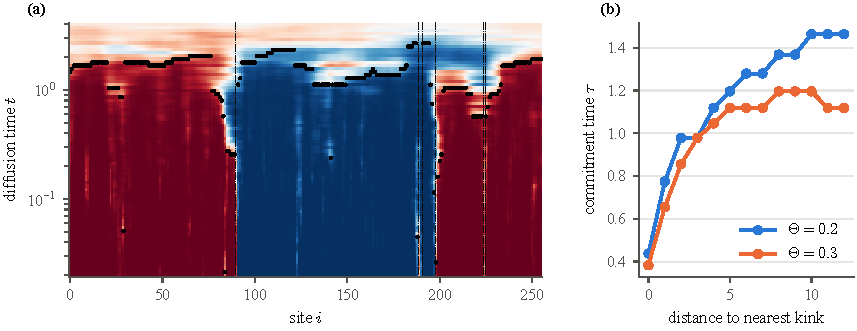
\includegraphics[width=\textwidth]{fig5-speciation.pdf}
\caption{(a) Polarisation $2P(a_i>0\mid\vx_t)-1$ of one chain at $\Theta=0.2$ ($\xi=19.5$ sites), red positive and blue negative;
dots, commitment times; dotted lines, kinks of the clean chain. (b) Median commitment time against the distance to the nearest
kink, domains of at least 8 sites, 32 chains per temperature.}
\label{fig:speciation}
\end{figure}

\end{document}
